\chapter{Numerical experiments and simulation results}

\section{Statistics from the model}
The model developed thus far is a numerical framwork for simulating growing cell colonies.
There is an element of randomness in the model: when two nodes are dislodged from the 
same point there is initially no preferred direction to move in so one must be chosen randomly
before other forces can take effect. For this reason, every seperate run of the model 
starting with identical initial conditions will look very different after time has passed. 
It is expected however that some ``averaged''
quantity will stabilise so long as the model is simulated over a fairly large number of runs.
Seperate runs of the model belong to a set called an ensemble.
We will start with a relatively straightforward metric, the number of cells at time
$T = 500$ steps.
\\

A fully grown colony will in general not be perfectly circular in shape.
 In order to measure the roundness of the colony we use the compactness metric used for 
 roundness in image processing (quote Kai use of this metric)
\begin{equation}
  C = \frac{P^2}{4 \pi A},
\end{equation}
where $C \in [1, \infty)$ is $1$ for a circle and can get to large numbers for 
highly branching shapes, $A$ is the colony area, and $P$ is the colony perimeter. 
Both of these are calculated from the formula for the microscopic cell
density which is always given by when $f(x,y,t)$ changes sign. A black and white image 
is produced at each time step using Matlab's function \codeword{bwboundaries} as per
Kai's suggestion. The area then is given by summing up the grid squares that are
inside the implicit shape givcen by $f$ and multiplying by $h^2$. The perimeter
is got by using \codeword{bwboundaries}, which outputs an array of points on the boundary
from which the Euclidean distance between neighbouring points is found and then summed over.
\begin{figure}[!htb]
    \centering
    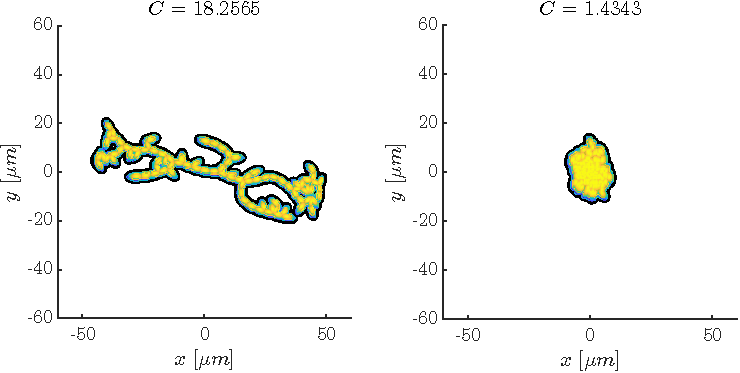
\includegraphics[width=\textwidth]{chapter1/figures/compareCompactness.pdf}
    \caption{A comparsion of high and low compactness}
    \label{fig:compatness_comparison}
\end{figure}

\begin{figure}[!htb] %Change this to [p] maybe ?
    \centering
    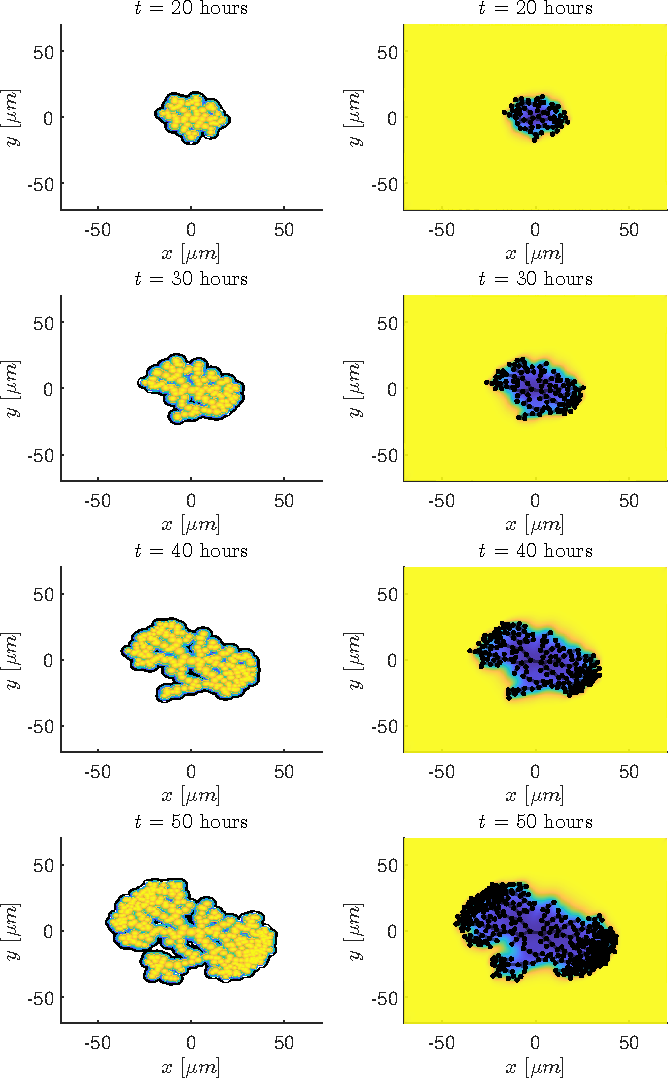
\includegraphics[width= 0.7\textwidth]{
        chapter2/figures/t_all__L1_0o10_L2_1o00_L3_1o00_L4_0o50_L5_1o00_L6_0o50_L7_1o00.pdf}
    \caption{A cell colony with parameter values given by
             $\lambda_1 = 0.1$,  
             $\lambda_2 = 1.0$, 
             $\lambda_3 = 1.0$, 
             $\lambda_4 = 0.5$, 
             $\lambda_5 = 1.0$, 
             $\lambda_6 = 0.5$, 
             $\lambda_7 = 1.0$. 
             On the left we have the biomass field, the nutrient field is on the right.}
    \label{fig: sdsd}
\end{figure}


\newpage


\begin{figure}[!htb] %Change this to [p] maybe ?
    \centering
    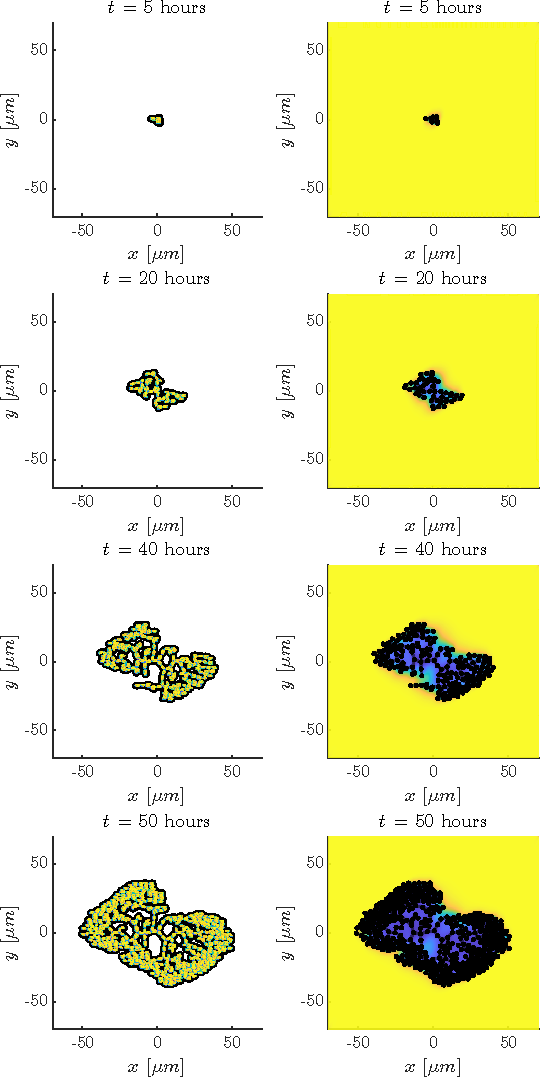
\includegraphics[width= 0.7\textwidth]{
        chapter2/figures/t_all_L1_0o10_L2_5o00_L3_1o00_L4_0o50_L5_1o00_L6_2o00_L7_0o50.pdf}
    \caption{A cell colony with parameter values given by
             $\lambda_1 = 0.1$,  
             $\lambda_2 = 5.0$, 
             $\lambda_3 = 1.0$, 
             $\lambda_4 = 0.5$, 
             $\lambda_5 = 1.0$, 
             $\lambda_6 = 2.0$, 
             $\lambda_7 = 0.5$. 
             Biomass on left and nutrient field on the right.}
    \label{fig: sdsd}
\end{figure}

\newpage

\begin{figure}[!htb] %Change this to [p] maybe ?
    \centering
    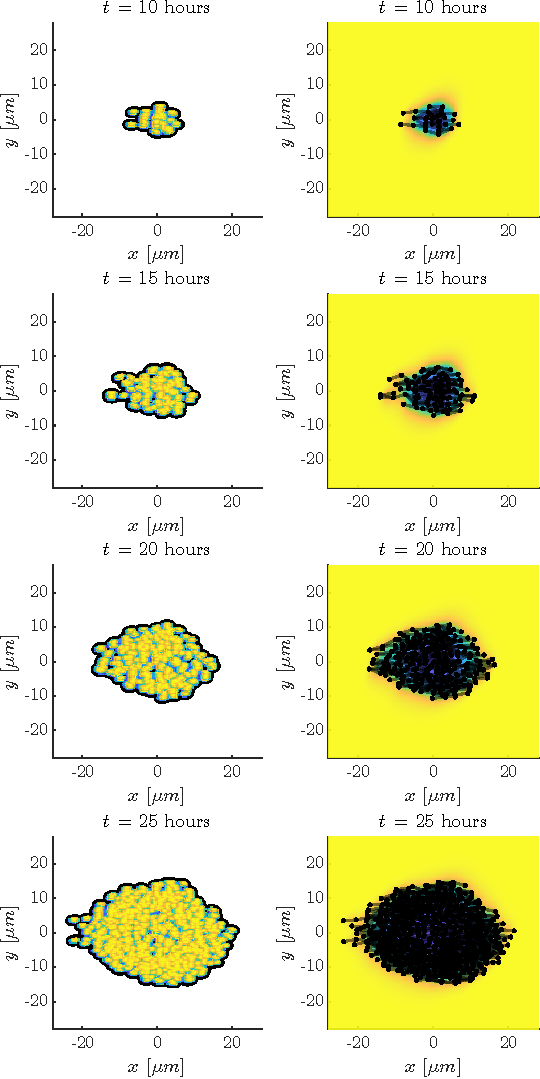
\includegraphics[width= 0.7\textwidth]{
        chapter2/figures/t_all__L1_0o10_L2_5o00_L3_1o00_L4_0o50_L5_1o00_L6_0o40_L7_0o60.pdf}
    \caption{A cell colony with parameter values given by
             $\lambda_1 = 0.1$,  
             $\lambda_2 = 5.0$, 
             $\lambda_3 = 1.0$, 
             $\lambda_4 = 0.5$, 
             $\lambda_5 = 1.0$, 
             $\lambda_6 = 0.4$, 
             $\lambda_7 = 0.6$. 
             Biomass on left and nutrient field on the right.}
    \label{fig: sdsd}
\end{figure}

\begin{figure}[!htb] %Change this to [p] maybe ?
    \centering
    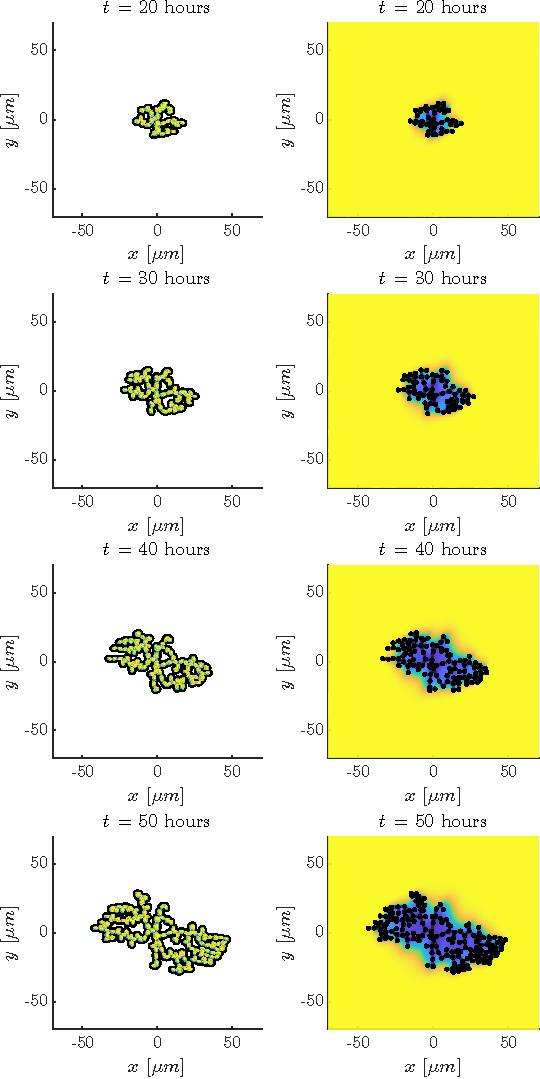
\includegraphics[width= 0.7\textwidth]{
        chapter2/figures/t_all__L1_0o10_L2_5o00_L3_1o00_L4_0o50_L5_1o00_L6_2o00_L7_0o60.pdf}
    \caption{A cell colony with parameter values given by
             $\lambda_1 = 0.1$,  
             $\lambda_2 = 5.0$, 
             $\lambda_3 = 1.0$, 
             $\lambda_4 = 0.5$, 
             $\lambda_5 = 1.0$, 
             $\lambda_6 = 2.0$, 
             $\lambda_7 = 0.6$. 
             Biomass on left and nutrient field on the right.}
    \label{fig: sdsd}
\end{figure}




\begin{figure}[!htb] %Change this to [p] maybe ?
    \centering
    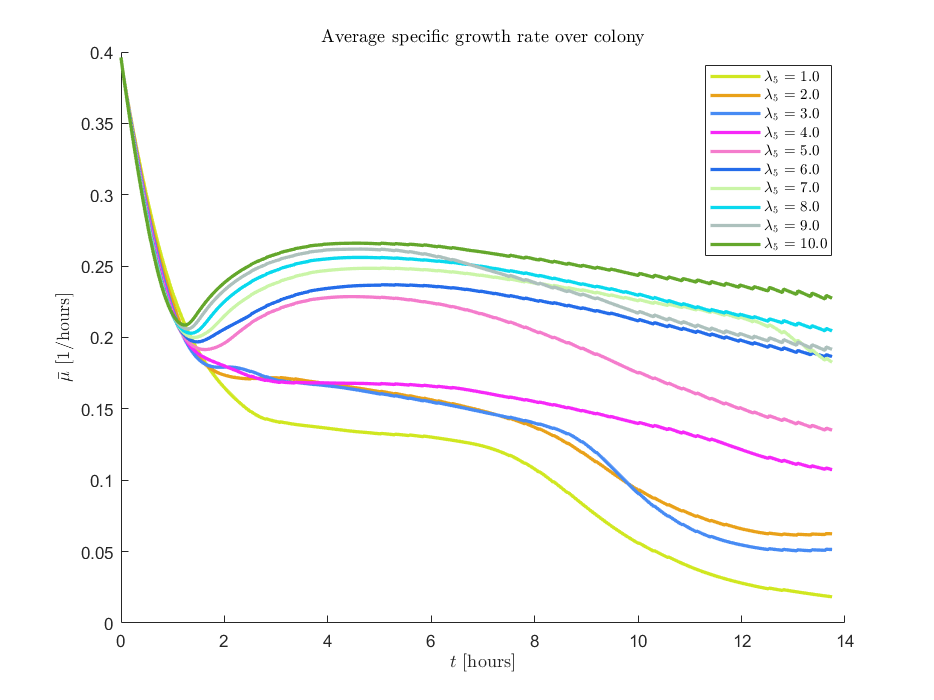
\includegraphics[width= 1\textwidth]{
        chapter2/figures/SpecificGrowthRatePlot.png}
    \caption{The colony average specific growth rate for different values of $\lambda_5$
                is measured and plotted over time for ensemble size $1$. The rest of the parameters 
                took the values:
                $\lambda_1 = 0.1$,  
                $\lambda_2 = 1.0$, 
                $\lambda_3 = 1.0$, 
                $\lambda_4 = 1.0$, 
                $\lambda_5$ (variable), 
                $\lambda_6 = 0.5$, 
                $\lambda_7 = 0.7$.
                Remarkably, when $\lambda_5 \geq 5.0$ there is an interesting dynamic that 
                occurs based on the compettition between nutrient consumption rate ($\lambda_6$)
                and the mobility ($\lambda_5$). For small values of mobility,
                the cells are not able to move enough into areas where the nutrient has not 
                decayed.}
    \label{fig:ColonySimulationNutrientFieldN210}
    \end{figure}
